\documentclass{standalone}

\usepackage{graphics}
\usepackage[dvipsnames,svgnames]{xcolor}

\usepackage{tikz,pgf,pgfplots,circuitikz}
\pgfplotsset{compat=1.15}
\usetikzlibrary{intersections,arrows.meta,angles,calc,3d,decorations.pathmorphing}

\usepackage{amssymb,amsfonts,amsthm,mathtools}
\usepackage{physics,braket,bm}

\begin{document}  
  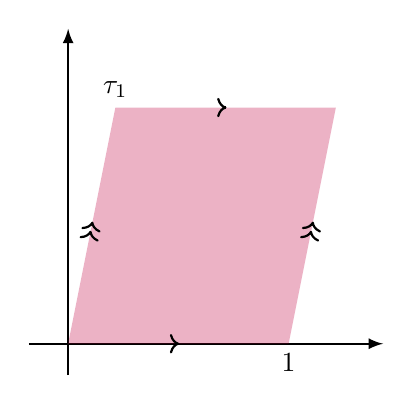
\begin{tikzpicture}[scale=1]
    \draw[-latex,thick](-0.5,0)--(4,0);
    \draw[-latex,thick](0,-0.4)--(0,4);

    \fill[purple,opacity=0.3](0,0)--(2.8,0)--(3.4,3.0)--(0.6,3.0);

    \draw(0.6,3.0)node[above]{$\tau_{1}$};
    \draw(2.8,0)node[below]{$1$};
    
    \draw[->,thick](1.4,0)--(1.41,0);
    \draw[->,thick](2.0,3)--(2.01,3);
    
    \draw[->>,thick](0.3,1.5)--(0.31,1.55);
    \draw[->>,thick](3.1,1.5)--(3.11,1.55);
  \end{tikzpicture}
\end{document}
